\section{Storage solutions}

During the 80s and 90s, data was primarily generated by humans. 
Today, machines produce data at an unprecedented pace.

Various forms of media, such as images, videos, audio files, and social media platforms, have emerged as significant sources of big data. 
The integration of Industry 4.0 technologies and Artificial Intelligence has further increased data production, ushering in a new era of data-centricity and innovation.

The trend now favors a centralized storage approach, which offers several advantages: reducing redundant data, streamlining storage efficiency, and automating replication and backup processes to ensure data reliability and security. 
This centralized model ultimately leads to reduced management costs.

Historically, HDDs have dominated the storage technology landscape, characterized by magnetic disks with mechanical interactions. 
However, recent advancements have introduced SSDs, which have no mechanical parts and are constructed using transistors, specifically NAND flash-based devices. 
Additionally, NVMe (Non-Volatile Memory Express) has emerged as the latest industry standard. Despite these innovations, tapes persist as a reliable storage solution.

Certain large storage servers employ SSDs as caches for multiple HDDs. 
Similarly, some latest-generation motherboards integrate a small SSD with a larger HDD to enhance disk speed. 
Additionally, certain HDD manufacturers produce Solid State Hybrid Disks (SSHDs), combining a small SSD with a large HDD within a single unit.

From the perspective of an OS, disks are viewed as collections of data blocks that can be read or written independently.
To facilitate their organization and management, each block is assigned a unique numerical address known as the Logical Block Address (LBA). 
The OS typically groups these blocks into clusters, which are the smallest units the OS can read from or write to on a disk.
Cluster sizes typically range from one disk sector (512 bytes) to 128 sectors (64 kilobytes).
\begin{figure}[H]
    \centering
    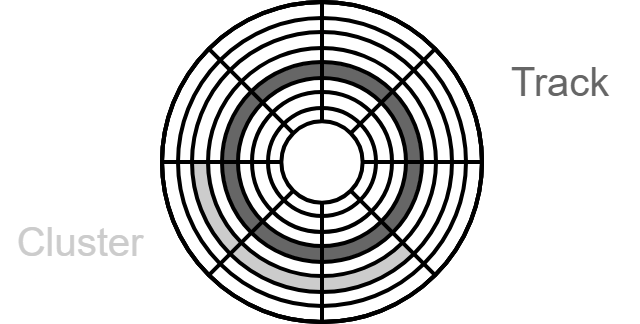
\includegraphics[width=0.5\linewidth]{images/hdd.png}
    \caption{HDD structure}
\end{figure}
Clusters encompass two crucial components:
\begin{enumerate}
    \item \textit{File data}: The actual content stored within files.
    \item \textit{Metadata}: Essential information supporting the file system, including:
        \begin{itemize}
            \item File names.
            \item Directory structures and symbolic links.
            \item File size and type.
            \item Creation, modification, and last access dates.
            \item Security information such as owners, access lists, and encryption details.
            \item Links to the LBA where the file content is located on the disk.
        \end{itemize}
\end{enumerate}
Hence, the disk can harbor various types of clusters:
\begin{itemize}
    \item \textit{Fixed-position metadata}: reserved to bootstrap the entire file system.
    \item \textit{Variable-position metadata}: used to store the folder structure.
    \item \textit{File data}: housing the actual content of files.
    \item \textit{Unused space}: available to accommodate new files and folders.
\end{itemize}

To read a file, the process involves:
\begin{enumerate}
    \item Accessing the metadata to locate its blocks
    \item Accessing the blocks to read its content
\end{enumerate}

Writing a file involves:
\begin{enumerate}
    \item Accessing the metadata to locate free space
    \item Writing the data into the assigned blocks
\end{enumerate}
Since the file system operates on clusters, the actual space occupied by a file on a disk is always a multiple of the cluster size, denoted by $c$. 
This is given by the formula:
\[a=\left\lceil \dfrac{s}{c} \right\rceil\cdot c\]
Here, $a$ is the actual size on disk, $s$ is the file size, and $c$ is the cluster size.
The wasted disk space, $w$, due to organizing the file into clusters can be computed as:
\[w=a-s\]
This unused space is referred to as the internal fragmentation of files.
\begin{example}
    Let's consider a hard disk with a cluster size of eight bytes and a file with a size of twenty-seven bytes. 
    The actual size on the disk would be:
    \[a=\left\lceil \dfrac{s}{c} \right\rceil\cdot c=\left\lceil \dfrac{27}{8} \right\rceil\cdot 8=32\:\text{B}\]
    And the wasted disk space would be:
    \[w=a-s=32-27=5\:\text{B}\]
\end{example}

Deleting a file involves updating the metadata to indicate that the blocks previously allocated to the file are now available for use by the OS. 
However, this process does not physically remove the data from the disk; the data remains intact until new data is written to the same clusters, overwriting the old data.

As the disk's lifespan progresses, there may not be sufficient contiguous space available to store a file. 
In such instances, the file is divided into smaller chunks and distributed across free clusters scattered throughout the disk.
This process of splitting a file into non-contiguous clusters is known as external fragmentation, which can significantly degrade the performance of a Hard Disk Drive (HDD).

\subsection{Hard Disk Drive}
A Hard Disk Drive (HDD) utilizes rotating disks (platters) coated with magnetic material for data storage. 
Information can be accessed randomly, allowing for the storage or retrieval of individual data blocks in any order, rather than sequentially. 
The HDD comprises one or more rigid rotating disks with magnetic heads positioned on a moving actuator arm, facilitating the reading and writing of data onto the surfaces.
\begin{figure}[H]
    \centering
    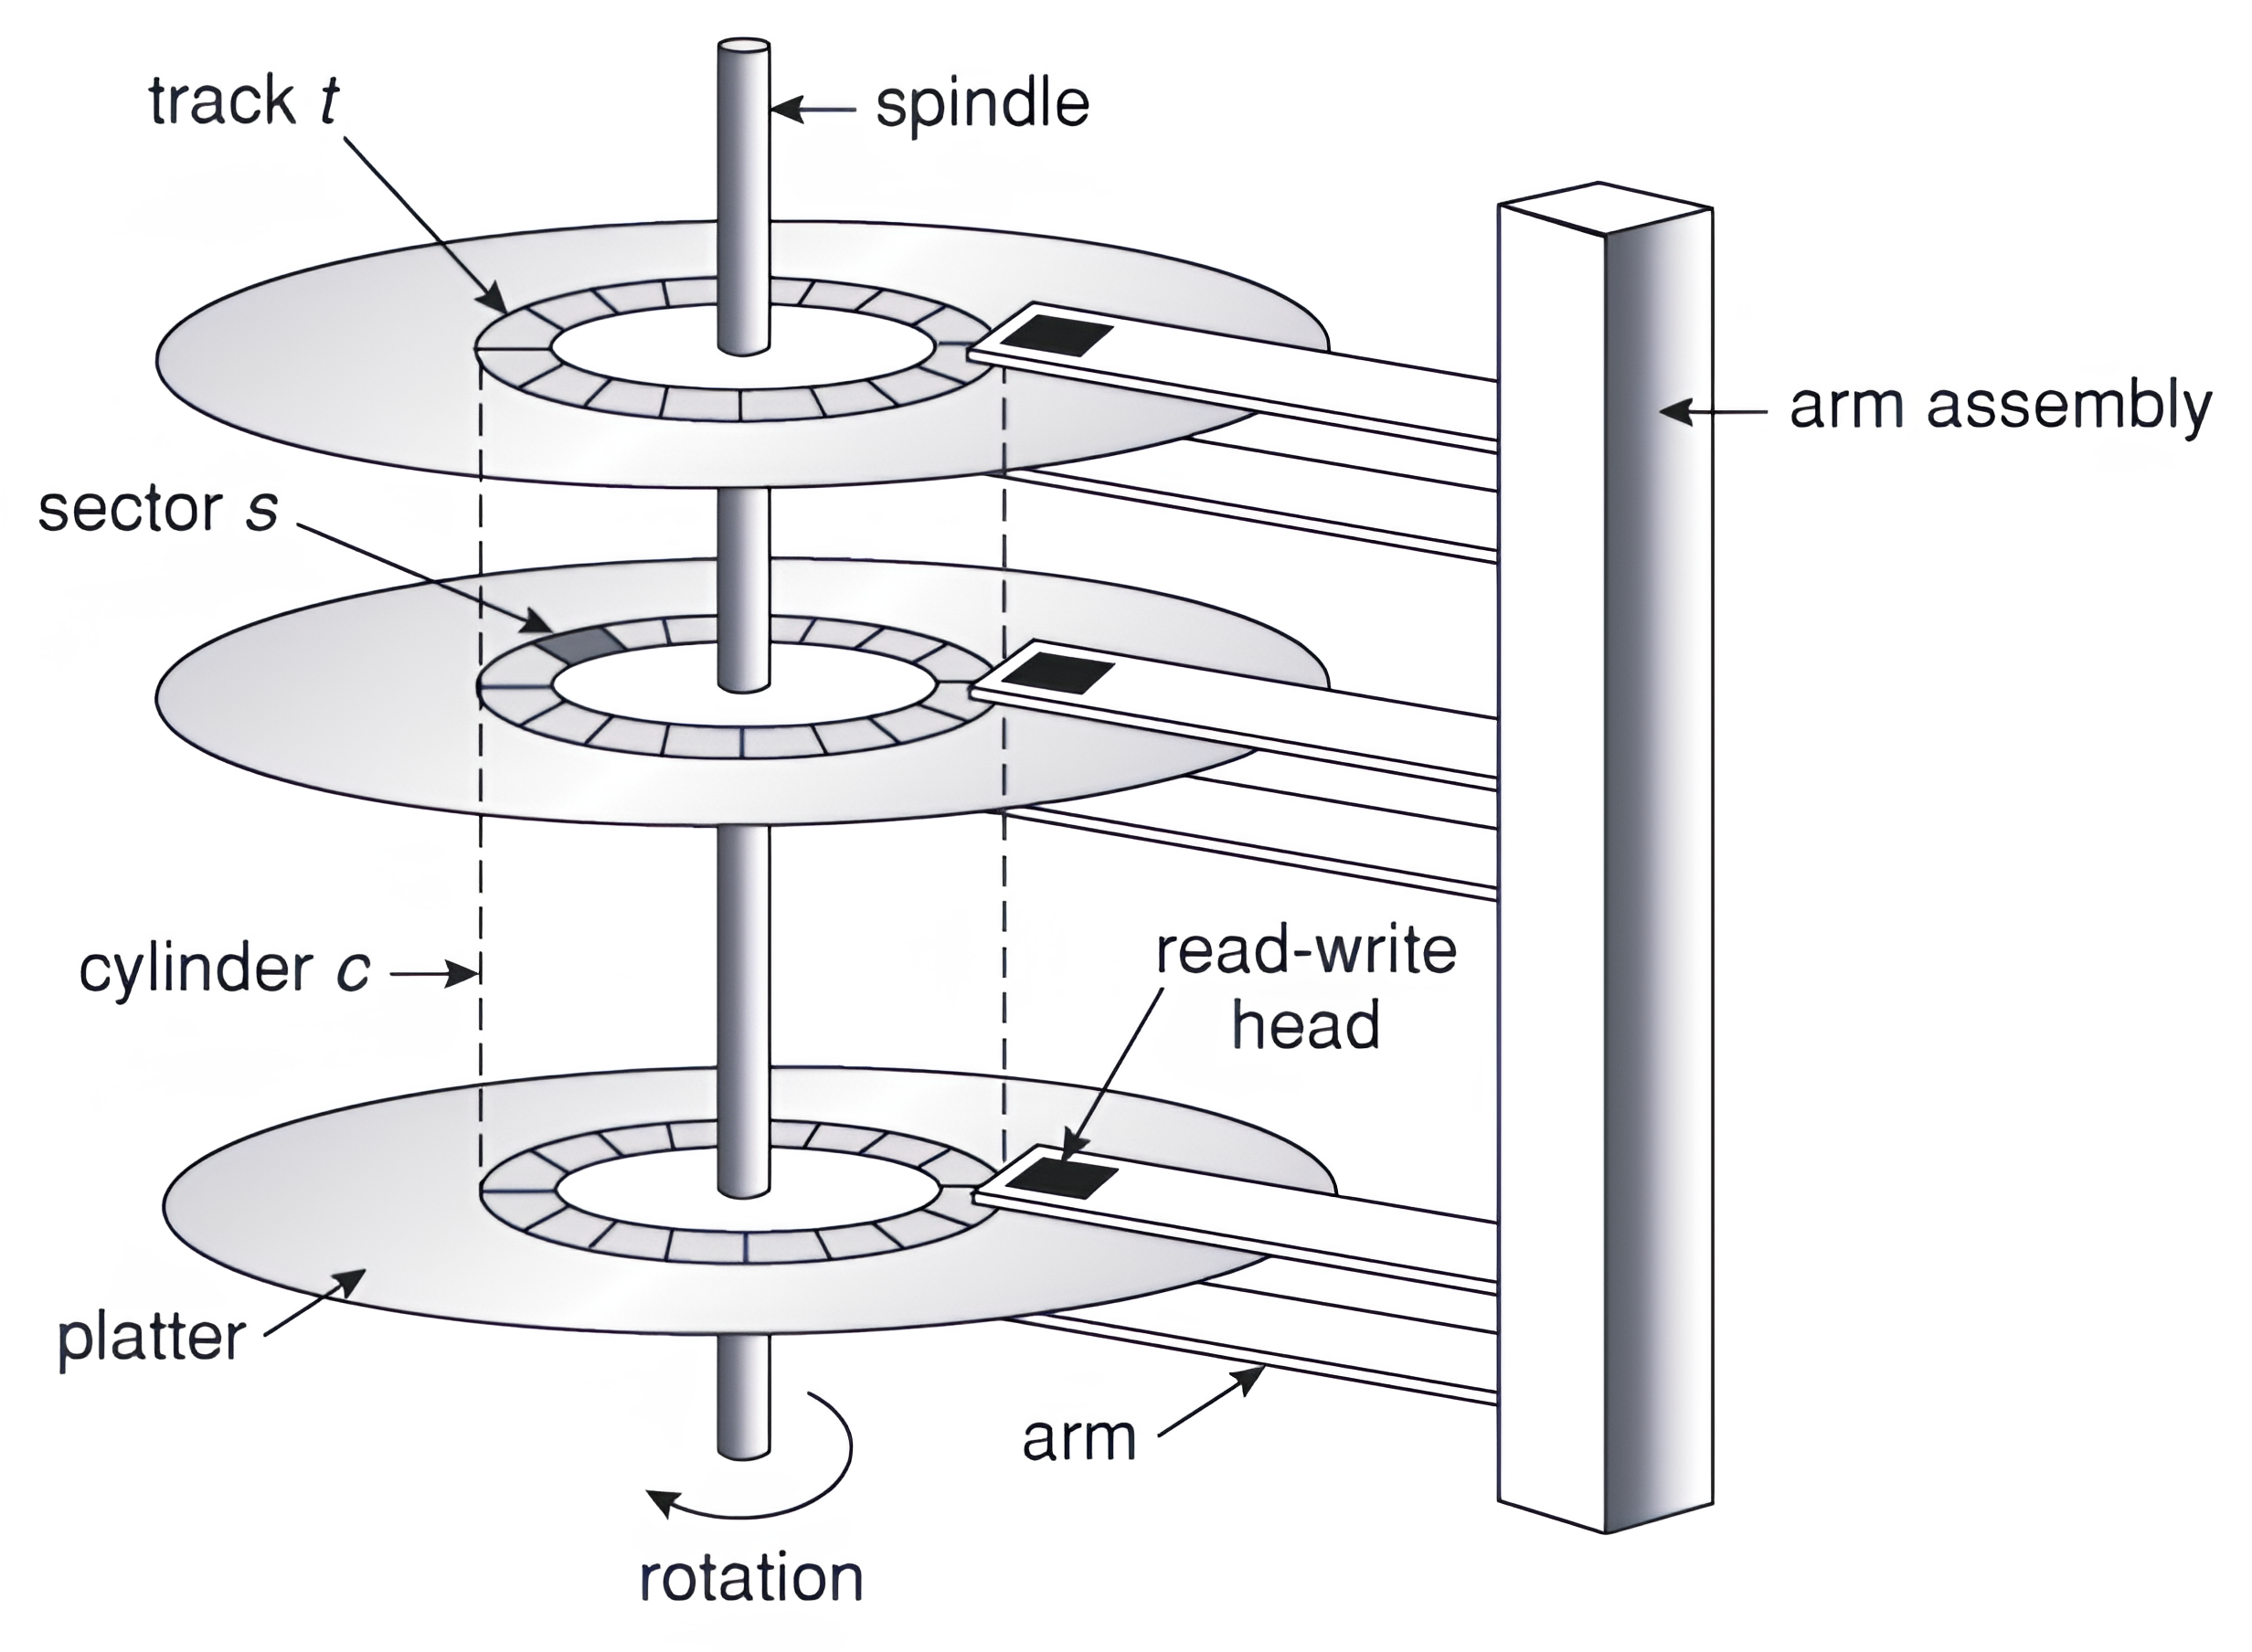
\includegraphics[width=0.5\linewidth]{images/hdds.png}
    \caption{HDD structure}
\end{figure}
Externally, HDDs present a multitude of blocks. Each sector write is indivisible and includes a header along with an error correction code. 
However, writing multiple sectors can be interrupted, resulting in a torn write scenario, where only part of a multi-sector update is successfully written to the disk.

Regarding drive geometry, sectors are organized into tracks, with a cylinder representing a specific track across multiple platters. 
These tracks are arranged in concentric circles on the platters, and a disk may consist of multiple double-sided platters. 
The drive motor maintains a constant rate of rotation for the platters, typically measured in Revolutions Per Minute (RPM).

Present-day technology specifications include:
\begin{itemize}
    \item \textit{Diameter}: approximately 9 cm (3.5 inches), accounting for two surfaces.
    \item \textit{Rotation speed}: ranges from 7200 to 15000 RPM.
    \item \textit{Track density}: reaching up to 16,000 Tracks Per Inch (TPI).
    \item \textit{Heads}: can be parked either close to the center or towards the outer diameter, particularly in mobile drives.
    \item \textit{Disk buffer cache}: embedded memory within a HDD, serving as a buffer between the disk and the computer.
\end{itemize}

\paragraph*{Cache}
Numerous disks integrate caches, often referred to as track buffers, which typically consist of a small amount of RAM.
These caches serve several purposes:
\begin{enumerate}
    \item \textit{Read caching}: this minimizes read delays caused by seeking and rotation.
    \item \textit{Write caching}: there are two primary types of write caching:
        \begin{itemize}
            \item \textit{Write back cache}: in this mode, the drive acknowledges writes as complete once they have been cached. 
                However, this feature can be risky as it may lead to an inconsistent state if power is lost before the write back event.
            \item \textit{Write through cache}: here, the drive acknowledges writes as complete only after they have been written to the disk.
        \end{itemize}
\end{enumerate}

\paragraph*{Standard disk interfaces}
The standard disk interfaces are: 
\begin{itemize}
    \item \textit{ST-506}: ancient standard characterized by commands and addresses in stored in device registers.
    \item \textit{Advanced Technology Attachment} (ATA): standardized as Integrated Drive Electronics (IDE).
    \item \textit{Integrated Drive Electronics} (IDE): used primarily in older systems.
    \item \textit{Serial Advanced Technology Attachment} (SATA): current standard for connecting storage devices.
    \item \textit{SCSI}: a packet-based interface with devices translating LBA to internal formats.
        It is transport-independent and utilized in various devices including USB drives.
    \item \textit{iSCSI}: a variant of SCSI over TCP/IP and Ethernet.
\end{itemize}

\paragraph*{Transfer time}
With HDD we can have four types of delay: 
\begin{itemize}
    \item \textit{Rotational delay}: time it takes for the desired sector to rotate under the read head. 
        It's influenced by the disk's rotational speed, measured in RPM.
        The full rotation delay is calculated as: 
        \[R=\dfrac{1}{RPM_{\text{Disk}}}\]
        While the average rotation time is typically half of the full rotation delay, given by: 
        \[T_{R}=\dfrac{60\cdot R}{2}\]
        in seconds.
    \item \textit{Seek delay}: refers to the time it takes for the read head to move to a different track on the disk. 
        The seek time includes components such as acceleration, coasting, deceleration, and settling. 
        Modeling seek time with a linear dependency on distance, we find that the average seek time $T_{S_{avg}}$ is one-third of the maximum seek time $T_{S_{\max}}$. 
    \item \textit{Transfer time}: time required to read or write bytes of data from or to the disk. 
    \item \textit{Controller overhead}: additional time incurred for managing the requests sent to the disk controller.
        It involves tasks such as buffer management for data transfer and the time taken to send interrupts.
\end{itemize}
The service time, also known as input output time, is determined by summing up various elements:
\[T_{I/O}=T_{S}+T_{R}+T_{T}+T_{C}\]
\begin{example}
    Let's consider a hard disk with the following specifications: a read and write sector size of $512$ bytes ($0.5\text{ KB}$), a data transfer rate of $50$ MB/s, a rotation speed of $10000$ RPM, a mean seek time of $6\text{ ms}$, and an overhead controller time of $0.2\text{ ms}$.
    The service time is calculated as:
    \[T_{I/O}=T_{S}+T_{R}+T_{T}+T_{C}=6+T_{R}+T_{T}+0.2\]
    Given:
    \[T_{R}=60\cdot\dfrac{1000}{2 \cdot RPM_{\text{Disk}}}=60\cdot\dfrac{1000}{2 \cdot 10000}=3.0\text{ ms}\]
    \[T_{T}=0.5\cdot\dfrac{1000}{50 \cdot 1024}=0.01\text{ ms}\]
    Hence:
    \[T_{I/O}=6+T_{R}+T_{T}+0.2=6+3+0.01+0.2=9.21\text{ ms}\]
\end{example}
The previous analysis of service times reflects a highly pessimistic scenario, assuming the worst-case conditions where disk sectors are extensively fragmented. 
This scenario occurs when files are tiny, typically occupying just one block, or when the disk suffers from significant external fragmentation. 
Consequently, each access to a sector necessitates both rotational latency and seek time.

However, in many practical situations, these extreme conditions are not encountered. 
Files tend to be larger than a single block and are stored contiguously, mitigating the need for frequent seeks and rotational latency.

We can assess the data locality of a disk by quantifying the percentage of blocks that can be accessed without requiring seek or rotational latency: 
\[T_{I/0}=(1-D_L)(T_{S}+T_{R})+T_{T}+T_{C}\]
\begin{example}
    Let's revisit the previous scenario but now with a data locality of $75\%$. 
    In this case, the time is computed as:
    \[T_{I/0}=(1-D_L)(T_{S}+T_{R})+T_{T}+T_{C}=(0.25)(6+3)+0.01+0.2=2.46\text{ ms}\]
    Here, DL represents the data locality factor. 
    Substituting the given values, we find the resulting time to be $2.46\text{ ms}$.
\end{example}

\paragraph*{Disk scheduling}
Caching is instrumental in enhancing disk performance, although it cannot fully compensate for inadequate random access times. 
The core concept lies in reordering a queue of disk requests to optimize performance. 
Estimating the request length becomes viable by considering the data's position on the disk.
Various scheduling algorithms facilitate this optimization process:
\begin{itemize}
    \item \textit{First Come First Served} (FCFS): this is the most basic scheduler, serving requests in the order they arrive. 
        However, it often results in a significant amount of time being spent seeking.
    \item \textit{Shortest Seek Time First} (SSTF): this scheduler minimizes seek time by always selecting the block with the shortest seek time. 
        SSTF is optimal and relatively easy to implement, but it may suffer from starvation.
    \item \textit{SCAN}, also known as the elevator algorithm: in SCAN, the head of the disk sweeps across the disk, servicing requests in a linear order. 
        This approach offers reasonable performance and avoids starvation, but average access times are higher for requests at the extremes of the disk.
    \item \textit{C-SCAN}: Similar to SCAN, but it only services requests in one direction, providing fairer treatment to requests. 
        However, it typically exhibits worse performance compared to SCAN.
    \item \textit{C-LOOK}: this is akin to C-SCAN, but with a twist: the head of the disk only moves as far as the last request in the queue, effectively reducing the range of movement.
\end{itemize}
These scheduling algorithms can be implemented in various ways:
\begin{itemize}
    \item \textit{OS scheduling}: requests are reordered based on LBA. 
        However, the OS lacks the ability to account for rotation delay.
    \item \textit{On-disk scheduling}: the disk possesses precise knowledge of the head and platter positions, allowing for the implementation of more advanced schedulers. 
        However, this approach requires specialized hardware and drivers.
    \item \textit{Disk command queue}: found in all modern disks, this queue stores pending read/write requests, known as Native Command Queuing (NCQ). 
        The disk may reorder items in the queue to enhance performance.
\end{itemize}

\subsection{Solid State Drive}
Solid State Drive (SSD), in contrast to traditional HDD, do not contain any mechanical or moving parts. 
Instead, they are constructed using transistors, similar to memory and processors. 
Unlike typical RAM, they can retain information even in the event of power loss.
These devices include a controller and one or more solid-state memory components. 
They are designed to utilize traditional HDD interfaces and form factors, although this may be less true as technology evolves. 
Furthermore, they offer higher performance compared to HDDs.

An SSD's components are arranged in a grid structure. 
Each cell within this grid can store varying amounts of data.
In particular, the memory is structured into pages and blocks. 
Each page contains several LBA, while a block generally comprises multiple pages, collectively holding approximately $128\text{ KB}$ and $256\text{ KB}$ of data: 
\begin{itemize}
    \item \textit{Blocks}: smallest units that can be erased, typically consisting of multiple pages. 
    \item \textit{Pages}: these are the smallest units that can be read or written. 
        Pages can exist in three states:
        \begin{itemize}
            \item \textit{Empty} (or ERASED): these pages do not contain any data.
            \item \textit{Dirty} (or INVALID): these pages contain data, but this data is either no longer in use or has never been used.
            \item \textit{In use} (or VALID): these pages contain data that can be read.
        \end{itemize}
\end{itemize}
Pages that are empty are the only ones that can be written to. 
Erasing is limited to pages that are dirty, and this must occur at the block level, where all pages within the block must be dirty or empty. 
Reading is only meaningful for pages in the valid state. 
If there are no empty pages available, a dirty page must be erased. 
If there are no blocks containing only dirty or empty pages available, special procedures should be followed to gather empty pages across the disk.
Resetting the original voltage to neutral is necessary before applying a new voltage to erase the value in flash memory. 

It's worth noting that while writing and reading a single page of data from an SSD is possible, an entire block must be deleted to release it.
This discrepancy is one of the underlying causes of the write amplification issue. 
Write amplification occurs when the actual volume of data physically written to the storage media is a multiple of the intended logical amount.
\begin{example}
    Let's examine an SSD with these specifications: page size of $4\text{ KB}$, block size of five pages, drive size of one block, read speed of $2$ KB/s, and write speed of $1$ KB/s.
    
    First, let's write a $4\text{ KB}$ text file to the brand-new SSD.
    The overall writing time will be $4$ seconds.

    Next, let's write a $8\text{ KB}$ picture file to the almost brand-new SSD.
    The overall writing time will be $8$ seconds.

    Now, suppose the text file in the first page is no longer needed.

    Finally, let's write a $12\text{ KB}$ picture to the SSD.
    It will take $24$ seconds. 
    In this case, we need to perform the following steps:
    \begin{itemize}
        \item Read the block into the cache.
        \item Delete the page from the cache.
        \item Write the new picture into the cache.
        \item ERASE the old block on the SSD.
        \item Write the cache to the SSD.
    \end{itemize}
    The OS only thought it was writing $12\text{ KB}$ of data when, in fact, the SSD had to read $8\text{ KB}$ ($2$ KB/s) and then write $20\text{ KB}$ ($1$ KB/s), the entire block.
    The writing should have taken $12$ seconds but actually took $4 + 20 = 24$ seconds, resulting in a write speed of $0.5\text{ KB}/s$ instead of $1$ KB/s.
\end{example}
As time goes on, write amplification significantly diminishes the performance of an SSD. 
This degradation occurs due to the wear-out of flash cells, resulting from the breakdown of the oxide layer within the floating-gate transistors of NAND flash memory. 
During the erasing process, the flash cell is subjected to a relatively high charge of electrical energy.

Each time a block is erased, this high electrical charge progressively degrades the silicon material. 
After numerous write-erase cycles, the electrical characteristics of the flash cell start to deteriorate, leading to unreliability in operation.

The elements in an SSD are: 
\begin{itemize}
    \item \textit{Flash Transition Layer} (FTL): emulate the functionality of a traditional HDD for the OS. 
        The FTL manages data allocation and performs address translation efficiently to mitigate the effects of write amplification.
        One method used by the FTL to reduce write amplification is through a technique called Log-Structured FTL. 
        This involves programming pages within an erased block sequentially, from low to high pages.
    \item \textit{Garbage collector}: recycle pages containing old data (marked as dirty or invalid) and wear leveling to evenly distribute write operations across the flash blocks. 
        This ensures that all blocks within the device wear out at approximately the same rate.
        Garbage collection incurs significant costs due to the necessity of reading and rewriting live data. 
        Ideally, garbage collection should reclaim blocks composed entirely of dead pages. 
        The expense of garbage collection is directly related to the volume of data blocks requiring migration. 
        To address this challenge, several solutions can be implemented:
        \begin{itemize}
            \item Increase device capacity by over provisioning with extra flash storage.
            \item Postpone cleaning operations to less critical periods.
            \item Execute garbage collection tasks in the background during periods of lower disk activity.
        \end{itemize}
    \item \textit{Mapping Table}: to mitigate the costs associated with mapping, several approaches have been developed:
        \begin{itemize}
            \item \textit{Block-based mapping}: employing a coarser grain approach to mapping.
                This approach encounters a write issue: the FTL needs to read a significant amount of live data from the old block and transfer it to a new one.
            \item \textit{Hybrid mapping}: utilizing multiple tables for mapping.
                The FTL manages two distinct tables: log blocks for page-level mapping, and data blocks for block-level mapping.
                When searching for a specific logical block, the FTL consults both the page mapping table and the block mapping table sequentially.
            \item \textit{Page mapping combined with caching}: implementing strategies to exploit data locality and optimize mapping efficiency.
                The fundamental concept is to cache the active portion of the page-mapped FTL. 
                When a workload primarily accesses a limited set of pages, the translations for those pages are retained in the FTL memory. 
                This approach offers high performance without incurring high memory costs, provided that the cache can accommodate the required working set. 
                However, there is a potential overhead associated with cache misses.
        \end{itemize}
\end{itemize}

\paragraph*{Wear leveling}
The SSD memory's erase and write cycle is limited, leading to asymmetry in the cycles that can shorten the SSD's lifespan. 
It's essential for all blocks to wear out at a similar pace to maintain longevity.
While the Log-structured approach and garbage collection aid in spreading writes, blocks may still contain cold data. 
To address this, the FTL periodically reads all live data from these blocks and rewrites it elsewhere. 
However, wear leveling can increase the SSD's write amplification and reduce performance. 
A simple policy involves assigning each block an erase and write cycle counter, ensuring that the difference between the maximum and minimum erase and write cycles remains below a certain threshold, denoted as $e$.

\paragraph*{Summary}
SSDs are increasingly common in laptops, desktops, and datacenter servers, despite their higher cost compared to conventional HDDs. 
Flash memory has limitations, including a finite number of write cycles, shorter lifespan, and the need for error correcting codes and over-provisioning (extra capacity). 
SSDs also exhibit different read/write speeds compared to HDDs. 
Unlike HDDs, SSDs are not affected by data locality and do not require defragmentation.

The FTL is a crucial component of SSDs, responsible for tasks such as data allocation, address translation, garbage collection, and wear leveling. 
However, the controller often becomes the bottleneck for transfer rates in SSDs.

\subsection{Comparison}
To assess these two memory types, we can utilize two metrics:
\begin{itemize}
    \item \textit{Unrecoverable Bit Error Ratio} (UBER): this metric indicates the rate of data errors, expressed as the number of data errors per bits read.
    \item \textit{Endurance Rating}: measured in terabytes written, this indicates the total data volume that can be written into an SSD before it's likely to fail. 
        It represents the number of terabytes that can be written while still meeting the specified requirements.
\end{itemize}